\chapter{Data Driven Surrogate Signal Extraction for Dynamic PET} \label{sec:data_driven_surrogate_signal_extraction_results}
    \newpage
    
    \longsection{Data Driven Surrogate Signal Extraction for Dynamic PET Introduction}{sec:data_driven_surrogate_signal_extraction_results_introduction}
        This chapter of the thesis contains work performed in the domain of \gls{SS} extraction from dynamic \gls{PET} data. The first section of this chapter introduces preliminary work performed using the \gls{PCA} method, including ventures to improve its robustness to variation caused by tracer kinetics.
    
    \longsection{PCA Data Driven Surrogate Signal Extraction Methods for Dynamic PET}{sec:pca_data_driven_surrogate_signal_extraction_methods_for_Dynamic_pet}
        This section investigates \gls{DD} methods to extract \gls{SS} from dynamic \gls{PET}, in particular this section will discuss methods using \gls{PCA} and compare them to similar methods, from the literature, some of which use \gls{SAM}.
        
        \subsection{Introduction} \label{sec:pca_data_driven_surrogate_signal_extraction_methods_for_dynamic_pet_introduction}
            As discussed in~\Fref{sec:respiratory_motion_in_pet} and \Fref{sec:impact_of_tof_on_respiratory_motion_model_estimation_using_nac_pet} respiratory motion correction is beneficial in positron emission tomography. Respiratory motion reduces image resolution in \gls{PET} by introducing blurring and mis-alignment artefacts~\boxcite{Nehmeh2008a}. Methods of motion correction include gated reconstruction, where the acquisition is binned based on a respiratory trace. Gating requires a \gls{SS} which reflects the position the patient is in the respiratory cycle over time. Methods to determine \glss{SS} include those which use an external devices, like the \gls{RPM}. However, a disadvantage of these methods is that they require the use of additional equipment and a change to clinical practise. Thus, \gls{DD} methods to extract \glss{SS} have become an alternative, for more detail see~\Fref{sec:data_driven}. 
            
            However, data driven methods have the disadvantage that they are adversely affected by the tracer kinetics of a dynamic acquisition. Current \gls{DD} \gls{SS} extraction methods struggle with dynamic \gls{PET} data where the tracer kinetics, at the start of the acquisition, offer more variance than the respiratory motion does. Previously, a moving window based approach using \gls{SAM} was proposed~\boxcite{Schleyer2014}. \gls{PCA} is a dimensionality reduction technique which produces a series of eigenvectors and weights where the eigenvectors are the orthogonal vectors of descending variance through the data and the weights are the magnitude of the contribution of the components to the data. Thus the first eigenvector from \gls{PCA} will represent the vector of greatest variance through the data, in thoracic \gls{PET} this will usually be caused by the \gls{RM} of the patient, but is not always. This section seeks to evaluate several adaptions of the \gls{PCA} method through which it can be used with dynamic data. The methods explored in this section include using the use of a moving window, and re-use of the \glss{PC} from a later time point to estimate the \gls{SS} from earlier time points.
        
        \subsection{Methods} \label{sec:pca_data_driven_surrogate_signal_extraction_methods_for_dynamic_pet_methods}
            \begin{figure}
                \centering
                
                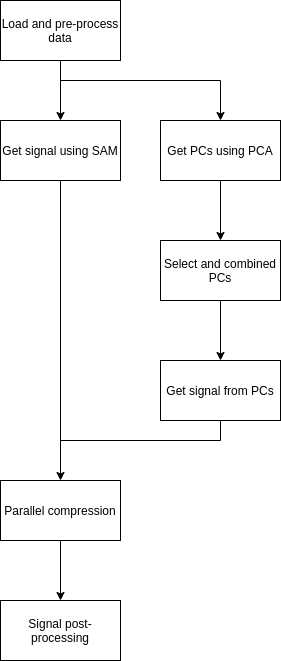
\includegraphics[width=0.6\linewidth]{figures/pca_data_driven_surrogate_signal_extraction_methods_for_dynamic_pet_methods_data_driven_surrogate_signal_extraction_overview.png}
                
                \captionsetup{singlelinecheck=false, justification=centering}
                \caption{A diagram showing an overview of the possible ways in which the method could be executed.}
                \label{fig:pca_data_driven_surrogate_signal_extraction_methods_for_dynamic_pet_methods_data_driven_surrogate_signal_extraction_overview}
            \end{figure}
            
            The following subsections will address the method with respect to the diagram seen in~\Fref{fig:pca_data_driven_surrogate_signal_extraction_methods_for_dynamic_pet_methods_data_driven_surrogate_signal_extraction_overview}.
            
            \subsection{Data Acquisition} \label{sec:pca_data_driven_surrogate_signal_extraction_methods_for_dynamic_pet_methods_data_acquisition}
                $21$ dynamic \gls{18F-FDG} acquisitions, with a \gls{FOV} covering the upper lung and heart, were acquired on a \gls{GE} Discovery $710$. Each acquisition lasted approximately \SI{20}{\minute} with the acquisition starting before injection of the radiotracer. \glss{SS} were acquired in parallel using a \gls{RPM}.
                
            \subsection{Data Preparation} \label{sec:pca_data_driven_surrogate_signal_extraction_methods_for_dynamic_pet_methods_data_preparation}
                \begin{figure}
                    \centering
                    
                    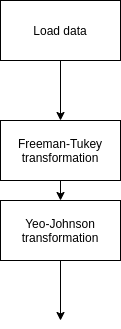
\includegraphics[width=0.4\linewidth]{figures/pca_data_driven_surrogate_signal_extraction_methods_for_dynamic_pet_methods_data_driven_surrogate_signal_extraction_input.png}
                    
                    \captionsetup{singlelinecheck=false, justification=centering}
                    \caption{A diagram showing the input to the method.}
                    \label{fig:pca_data_driven_surrogate_signal_extraction_methods_for_dynamic_pet_methods_data_driven_surrogate_signal_extraction_input}
                \end{figure}
                
                Data were unlisted into low spatial resolution sinograms, each with time frame duration of \SI{500}{\milli\second}, using the \gls{GE} PetToolbox following~\boxcite{Bertolli2018Data-DrivenTomography} resulting in sinograms with dimensions $95 x 16 x 47 x 11$ (radial positions $x$ angles $x$ transaxial plane $x$ \gls{TOF}). Data was pre-processed by first applying a Freeman-Tukey transformation~\boxcite{Freeman1950TransformationsRoot} before then applying a Yeo-Johnson power transformation~\boxcite{Yeo2000ASymmetry} this is in order to attempt to transform the Poisson distributed data to be more Gaussian-like. The Freeman-Tukey transformation was applied before the Yeo-Johnson power transformation as it was found that the Freeman-Tukey transformation made the Yeo-Johnson power transformation more reliable. Furthermore, it was also found that adding the Yeo-Johnson power transformation gave better results than the Freeman-Tukey transformation alone.
                
                The Freeman-Tukey transformation is defined as:

                \begin{equation} \label{eq:pca_data_driven_surrogate_signal_extraction_methods_for_dynamic_pet_methods_freeman_tukey}
                    S_g := \sqrt{S_p + 1} + \sqrt{S_p}
                \end{equation}

                \noindent where in~\Fref{eq:pca_data_driven_surrogate_signal_extraction_methods_for_dynamic_pet_methods_freeman_tukey} $S_g$ is the resultant, approximately Gaussian distributed, sinogram and $S_p$ is the original Poisson distributed sinogram $S_p$~\boxcite{Freeman1950TransformationsRoot}.
                
                The Yeo-Johnson power transformation is defined as:

                \begin{equation} \label{eq:pca_data_driven_surrogate_signal_extraction_methods_for_dynamic_pet_methods_yeo_johnson}
                    S_g := \begin{cases}
                                ((S_p + 1)^\lambda - 1) / \lambda                   & \quad \text{if } \lambda \neq 0 \text{, } S_p \geq 0 \\
                                \log(S_p + 1)                                       & \quad \text{if } \lambda = 0 \text{, } S_p \geq 0    \\
                                -[(-S_p + 1)^{(2 - \lambda)} - 1)] / (2 - \lambda)  & \quad \text{if } \lambda \neq 2 \text{, } S_p < 0    \\
                                -\log(-S_p + 1)                                     & \quad \text{if } \lambda = 2 \text{, } S_p < 0
                            \end{cases}
                \end{equation}

                \noindent where in~\Fref{eq:pca_data_driven_surrogate_signal_extraction_methods_for_dynamic_pet_methods_yeo_johnson} $S_g$ is the resultant, approximately Gaussian distributed, sinogram. The $\lambda$ parameter is determined by minimising the Kullback-Leibler distance between normal distributions and the transformed distribution~\boxcite{Yeo2000ASymmetry}. In the current implementation, a single $\lambda$ is determined from all of the data, although it would be feasible to find different $\lambda$ values for every element in the sinogram.
                
                A flowchart of the above can be seen in~\Fref{fig:pca_data_driven_surrogate_signal_extraction_methods_for_dynamic_pet_methods_data_driven_surrogate_signal_extraction_input}.
            
            \subsection{Surrogate Signal Extraction} \label{sec:pca_data_driven_surrogate_signal_extraction_methods_for_dynamic_pet_methods_surrogate_signal_extraction}
                \begin{figure}
                    \centering
                    
                    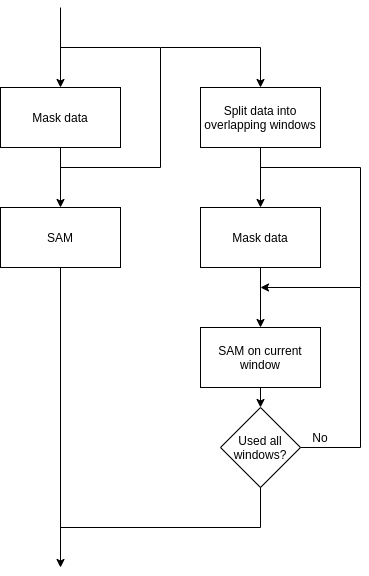
\includegraphics[width=0.9\linewidth]{figures/pca_data_driven_surrogate_signal_extraction_methods_for_dynamic_pet_methods_data_driven_surrogate_signal_extraction_sam.png}
                    
                    \captionsetup{singlelinecheck=false, justification=centering}
                    \caption{A diagram showing the \gls{SAM} branch of the method.}
                    \label{fig:pca_data_driven_surrogate_signal_extraction_methods_for_dynamic_pet_methods_data_driven_surrogate_signal_extraction_sam}
                \end{figure}
                
                \begin{figure}
                    \centering
                    
                    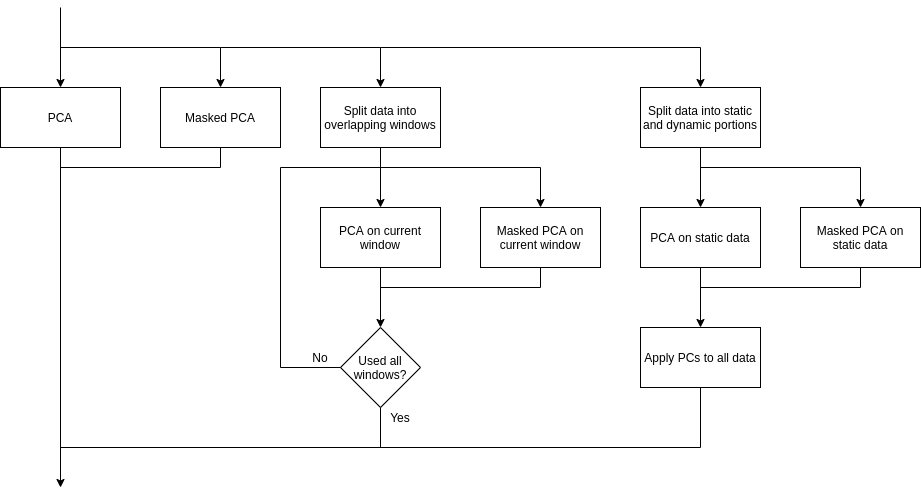
\includegraphics[width=1.0\linewidth]{figures/pca_data_driven_surrogate_signal_extraction_methods_for_dynamic_pet_methods_data_driven_surrogate_signal_extraction_pca.png}
                    
                    \captionsetup{singlelinecheck=false, justification=centering}
                    \caption{A diagram showing the \gls{PCA} branch of the method.}
                    \label{fig:pca_data_driven_surrogate_signal_extraction_methods_for_dynamic_pet_methods_data_driven_surrogate_signal_extraction_pca}
                \end{figure}
                
                \subsubsection{Pre-Processing} \label{sec:pca_data_driven_surrogate_signal_extraction_methods_for_dynamic_pet_methods_pre_processing}
                    Following the diagram in~\Fref{fig:pca_data_driven_surrogate_signal_extraction_methods_for_dynamic_pet_methods_data_driven_surrogate_signal_extraction_overview} the first major split in the method is between using \gls{PCA} or \gls{SAM}. \gls{SAM} is included, as mentioned previously in~\Fref{sec:pca_data_driven_surrogate_signal_extraction_methods_for_dynamic_pet_introduction}, as a comparison for the \gls{PCA} based methods. Thus, the \gls{SAM} based methods are less developed here to conform to literature, seen in~\boxcite{Schleyer2014}.
                    
                    Both the \gls{PCA} and \gls{SAM} based methods have the capacity for the input data to be Gaussian smoothed and further downsampled, different parameters are used for both methods. It has been found through experimentation that Gaussian smoothing can improve results, especially in the case of the \gls{SAM} methods. Further downsampling can be performed post smoothing to reduce memory usage, in this case linear interpolation has been found to be satisfactory and additionally is less computationally expensive to calculate than some methods, however Akima spline interpolation has been shown to give marginally improved results but is significantly more computationally expensive~\boxcite{Akima1970AProcedures}.
                        
                    Additionally, it had been found that the introduction of a mask to aid in the reduction of noise is beneficial. Both types of method can be used with a mask. The mask itself is defined as being true for any value in the sinogram above a predetermined threshold, values not in the mask are removed prior to further execution.
                
                \subsubsection{Applying PCA or SAM} \label{sec:pca_data_driven_surrogate_signal_extraction_methods_for_dynamic_pet_methods_applying_pca_or_sam}
                    Again, as can be seen from the diagram in~\Fref{fig:pca_data_driven_surrogate_signal_extraction_methods_for_dynamic_pet_methods_data_driven_surrogate_signal_extraction_overview} there are two methods of applying either \gls{PCA} or \gls{SAM} which are common to both routes.
                    
                    \begin{itemize}
                        \item Firstly there is what shall be referred to as the static method. Here, either \gls{PCA} or \gls{SAM} is applied to the entire data set in one go as it would be if the data were from a static acquisition, hence the name.
                        
                        \item Secondly there is the moving window method. Here the data is split into a series of windows, where each subsequent window overlaps with the previous window by half its length. The size of each window is predetermined and selected experimentally. \gls{PCA} or \gls{SAM} is applied independently on each window and the results are averaged together after sign correction as described now. The windows overlap as the sign of the signal from each window is arbitrary and the overlapping allows for a common sign to be found by comparing the \gls{CC} of neighbouring windows and flipping windows where the \gls{CC} is negative. The motivation for attempting the moving window method is to increase the relative importance of motion vs kinetics, this is achieved through small windows being used at early time points, where the tracer kinetics are at their most severe, and longer windows can be used at later time points. Smaller windows may help to extract \gls{RM} where they are shorter than the duration of the tracer kinetics.
                    \end{itemize}
                    
                    Additionally there is one method which has only been trialed with \gls{PCA}.
                    
                    \begin{itemize}
                        \item The one \gls{PC} method splits the data into two channels, one which only contains later time point data where the tracer kinetics have diminished and one which contains all the data. The cutoff between early and later time point data is determined experimentally. \gls{PCA} is applied to the later time point data only. The \glss{PC} from the later time point data can then be taken and multiplied by the channel containing all of the data to give the weights contributing to that \gls{PC} for all time points.
                        
                        The generic equation for calculating the weights (or signal) from the \gls{PC} and data is defined as:

                        \begin{equation} \label{eq:pca_data_driven_surrogate_signal_extraction_methods_for_dynamic_pet_methods_pc_weights}
                            W := PC * D
                        \end{equation}
        
                        \noindent where in~\Fref{eq:pca_data_driven_surrogate_signal_extraction_methods_for_dynamic_pet_methods_pc_weights} $W$ is the weights (or signal) found when multiplying the \gls{PC} $PC$ by data $D$.
                        
                        The motivation for attempting this method is that it was observed that \glss{PC} for late time point data didn't vary significantly when different windows were selected, however that was not true for early time point data. It could be hypothesised that because the \gls{RM} should be semi-consistent throughout the acquisition, then if a \gls{PC} is capturing the \gls{RM} at late time points then it should do the same at early time points.
                    \end{itemize}
                    
                    A flowchart of the above can be seen in~\Fref{fig:pca_data_driven_surrogate_signal_extraction_methods_for_dynamic_pet_methods_data_driven_surrogate_signal_extraction_sam} and~\Fref{fig:pca_data_driven_surrogate_signal_extraction_methods_for_dynamic_pet_methods_data_driven_surrogate_signal_extraction_pca}.
                
                \subsubsection{Selecting and Combining PCs} \label{sec:pca_data_driven_surrogate_signal_extraction_methods_for_dynamic_pet_methods_selecting_and_combining_pcs}
                    \begin{figure}
                        \centering
                        
                        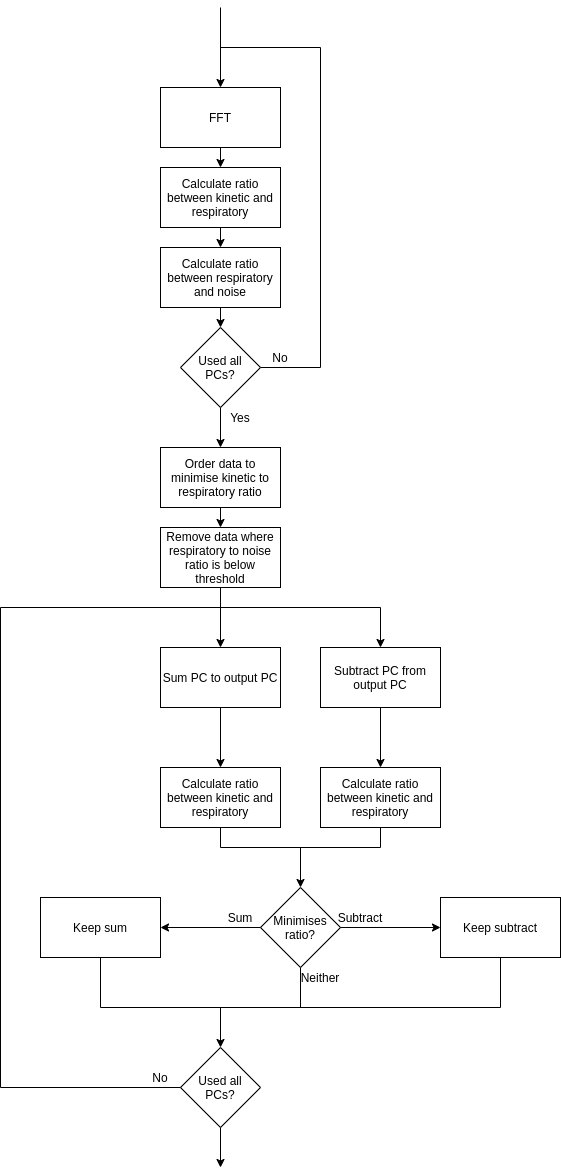
\includegraphics[width=0.7\linewidth]{figures/pca_data_driven_surrogate_signal_extraction_methods_for_dynamic_pet_methods_data_driven_surrogate_signal_extraction_select_combine.png}
                        
                        \captionsetup{singlelinecheck=false, justification=centering}
                        \caption{A diagram showing how \glss{PC} can be selected and combined.}
                        \label{fig:pca_data_driven_surrogate_signal_extraction_methods_for_dynamic_pet_methods_data_driven_surrogate_signal_extraction_select_combine}
                    \end{figure}
                
                    \begin{algorithm}
                        \caption{Get respiratory kinetic ratio and respiratory noise ratio}
                        \KwData{\glss{PC}}
                        \KwResult{respiratory kinetic ratio and respiratory noise ratio}
                        \;
                        $PSD$ := \gls{FFT} on current \gls{PC}\;
                        \;
                        $kineticContribution$ := mean of $PSD$ between \SI{0.0}{\hertz} and \SI{0.1}{\hertz}\;
                        $respiratoryContribution$ := mean of $PSD$ between \SI{0.1}{\hertz} and \SI{0.4}{\hertz}\;
                        $noiseContribution$ := mean of $PSD$ above \SI{0.4}{\hertz}\;
                        \;
                        $respiratoryKineticRatio$ := $respiratoryContribution$ / $kineticContribution$\;
                        $respiratoryNoiseRatio$ := $respiratoryContribution$ / $noiseContribution$\;
                        \;
                    \end{algorithm} \label{eq:pca_data_driven_surrogate_signal_extraction_methods_for_dynamic_pet_methods_selecting_and_combining_pcs_get respiratory_kinetic_ratio_and_respiratory_noise_ratio_pseudo_code}
                    
                    \begin{algorithm}
                        \caption{Selecting \glss{PC}}
                        \KwData{\glss{PC}}
                        \KwResult{selected \glss{PC}}
                        \;
                        \For{\gls{PC} in $PCs$}{
                            $RKRatio$, $RNRatio$ := get respiratory kinetic ratio and respiratory noise ratio from current \gls{PC}\;
                            \;
                            $RKRatioList$ append $RKRatio$\;
                            $RNRatioList$ append $RNRatio$\;
                        }
                        \;
                        remove \gls{PC} from $PCs$ where $RKRatioList$ \textless 1\;
                        remove \gls{PC} from $PCs$ where $RNRatioList$ \textless 1\;
                        \;
                        $PCs$ := $PCs$ * ($RKRatioList$ * $RNRatioList$)\;
                        order $PCs$\;
                    \end{algorithm} \label{eq:pca_data_driven_surrogate_signal_extraction_methods_for_dynamic_pet_methods_selecting_pcs_pseudo_code}
                    
                    \begin{algorithm}
                        \caption{Combining \glss{PC}}
                        \KwData{selected \glss{PC}}
                        \KwResult{respiratory \gls{PC}}
                        \;
                        $respiratoryPC$ := first \gls{PC} in $PCs$\;
                        remove $respiratoryPC$ from $PCs$\;
                        $RKRatio$, $RNRatio$ := get respiratory kinetic ratio and respiratory noise ratio from $respiratoryPC$\;
                        \;
                        \For{\gls{PC} in $PCs$}{
                            $sumPC$ := $respiratoryPC$ + current \gls{PC}\;
                            $subPC$ := $respiratoryPC$ - current \gls{PC}\;
                            \;
                            $sumRKRatio$, $sumRNRatio$ := get respiratory kinetic ratio and respiratory noise ratio from $sumPC$\;
                            $subtractRKRatio$, $subtractRNRatio$ := get respiratory kinetic ratio and respiratory noise ratio from $subtractPC$\;
                            \;
                            \eIf{$sumRKRatio$ \textgreater $RKRatio$}{
                                \uIf{$sumRNRatio$ \textgreater $RNRatio$}{
                                    $respiratoryPC$ := $sumPC$\;
                                    $RKRatio$ := $sumRKRatio$\;
                                    $RNRatio$ := $sumRNRatio$\;
                                }
                            }{
                                \uIf{$subtractRKRatio$ \textgreater $RKRatio$}{
                                    \uIf{$subtractRNRatio$ \textgreater $RNRatio$}{
                                        $respiratoryPC$ := $subtractPC$\;
                                        $RKRatio$ := $subtractRKRatio$\;
                                        $RNRatio$ := $subtractRNRatio$\;
                                    }
                                }
                            }
                        }
                    \end{algorithm} \label{eq:pca_data_driven_surrogate_signal_extraction_methods_for_dynamic_pet_methods_combining_pcs_pseudo_code}
                    
                    Furthermore, as an additional development of the previous methods a way to combine \glss{PC} was proposed. The motivation for this was that it could be observed that signals in the frequency window of \gls{RM} could be seen outside of the first few \glss{PC}. Additionally, a significant number of these had far less of a frequency contribution in the frequency window of the tracer kinetics. However, they may not be selected if only one \gls{PC} is used and determined by the greatest mean frequency contribution in the respiratory window, as in~\boxcite{Thielemans2011}, and~\boxcite{Bertolli2018Data-DrivenTomography}. This could lead to a reduced \gls{SNR}.
                    
                    In order to exploit those \glss{PC}, first the \gls{PSD} of each signal must be calculated using \gls{FFT}. These \gls{PSD} contain the frequency contribution of each signal between the frequencies of \SI{0.0}{\hertz} and \SI{1.0}{\hertz} (due to the frame duration). Next, frequency windows representing the content of information related to tracer kinetics, \gls{RM} and noise are defined. In the current implementation they are defined as \SI{0.0}{\hertz} to \SI{0.1}{\hertz}, \SI{0.1}{\hertz} to \SI{0.4}{\hertz} and above \SI{0.4}{\hertz} respectively. The contribution within each window is determined for each \gls{PC} by finding the mean magnitude within the windows. Ratios are then determined between the kinetic window and the respiratory window and the respiratory window and the noise window. Data are ordered such that the respiratory to kinetic window ratio is maximised, in other words the \gls{PC} which contributes the most respiratory information without contributing much kinetic information goes first. Any \gls{PC} where more noise is contributed than useful respiratory information, defined as a threshold on the noise to respiratory ratio, is then thrown away.
                    
                    In the order determined in the previous step the \glss{PC} are looped over and both summed and subtracted with a weighting (the respiratory to kinetic ratio multiplied by the respiratory to noise ratio for each \gls{PC}) and a new \gls{PSD} is found for both resulting signals. If one of the signals increases the respiratory frequency contribution more than the kinetic or noise contribution then it becomes the new best \gls{PC} and goes forward to the next iteration. \glss{PC} are both summed and subtracted to deal with the arbitrary sign problem mentioned earlier~\Fref{sec:pca_data_driven_surrogate_signal_extraction_methods_for_dynamic_pet_methods_applying_pca_or_sam}. A similar method of combining signals can be seen in~\boxcite{Kesner2010AMethods}, however the method presented here has the advantage over the method presented in~\boxcite{Kesner2010AMethods} as the metric to define a good signal here specifically looks to maximise a value related to the behaviour desired. However, in~\boxcite{Kesner2010AMethods} the standard deviation is maximised which could logically be increased through means other than those desired.
                    
                    Pseudo code for the above method can be seen in~\Fref{eq:pca_data_driven_surrogate_signal_extraction_methods_for_dynamic_pet_methods_selecting_and_combining_pcs_get respiratory_kinetic_ratio_and_respiratory_noise_ratio_pseudo_code}, ~\Fref{eq:pca_data_driven_surrogate_signal_extraction_methods_for_dynamic_pet_methods_selecting_pcs_pseudo_code} and~\Fref{eq:pca_data_driven_surrogate_signal_extraction_methods_for_dynamic_pet_methods_combining_pcs_pseudo_code}.
                    
                    A flowchart of the above can be seen in~\Fref{fig:pca_data_driven_surrogate_signal_extraction_methods_for_dynamic_pet_methods_data_driven_surrogate_signal_extraction_select_combine}.
                
                \subsubsection{Post-Processing} \label{sec:pca_data_driven_surrogate_signal_extraction_methods_for_dynamic_pet_methods_post_processing}
                    \begin{figure}
                        \centering
                        
                        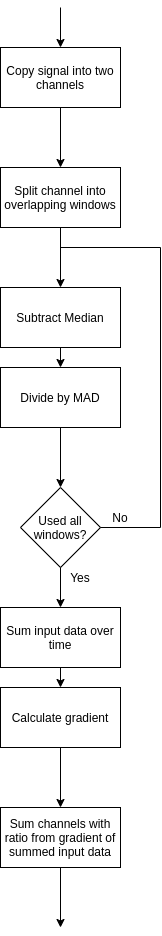
\includegraphics[width=0.2\linewidth]{figures/pca_data_driven_surrogate_signal_extraction_methods_for_dynamic_pet_methods_data_driven_surrogate_signal_extraction_parallel.png}
                        
                        \captionsetup{singlelinecheck=false, justification=centering}
                        \caption{A diagram showing the parallel compression method.}
                        \label{fig:pca_data_driven_surrogate_signal_extraction_methods_for_dynamic_pet_methods_data_driven_surrogate_signal_extraction_parallel}
                    \end{figure}
                    
                    \begin{figure}
                        \centering
                        
                        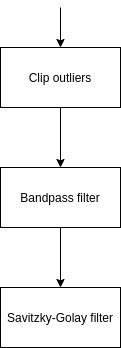
\includegraphics[width=0.5\linewidth]{figures/pca_data_driven_surrogate_signal_extraction_methods_for_dynamic_pet_methods_data_driven_surrogate_signal_extraction_output.png}
                        
                        \captionsetup{singlelinecheck=false, justification=centering}
                        \caption{A diagram showing the output of the method.}
                        \label{fig:pca_data_driven_surrogate_signal_extraction_methods_for_dynamic_pet_methods_data_driven_surrogate_signal_extraction_output}
                    \end{figure}
                    
                    Regardless of method used there is still some effects of the tracer kinetics to be expected at early time points and noise throughout. Thus a method of parallel compression has been proposed to deal with the remaining tracer kinetics and a plethora of smoothing to deal with the noise.
                    
                    \begin{itemize}
                        \item Firstly there is, what shall be referred to as, parallel compression. This is a method borrowed from audio engineering (appearing notably in Dolby A noise reduction) whereby the signal is split into two channels, one has its dynamic range decimated while the other passes unchanged before they are summed back together~\boxcite{Izhaki2012MixingTools}. This has the effect of reducing large differences in the dynamic range of the signal without losing a lot of breath to breath variability. In order to achieve this here the signal is split into two channels and one channel is further split into a series of small moving windows. The channel comprised of windows now has the median value of each window subtracted and each window divided by its \gls{MAD}. This channel then has its windows averaged back together before being combined with the unadulterated channel. The channels are combined following the gradient of the head count signal, the head count signal is the sum of the sinogram at each time point, this signal is normalised between zero and one and where it is larger more of the compressed signal is summed.
                        
                        \item Even though most of the large macro changes in intensity are dealt with by parallel compression some momentary spikes still make it through the process. Thus outliers are removed where they are outside a threshold of the quantile of the signal and new values are interpolated.
                        
                        \item Smoothing is applied first through the use of a bandpass filter before a Savitzky-Golay filter is applied. A Savitzky-Golay filter is a moving window polynomial filter~\boxcite{Savitzky1964SmoothingProcedures}. The parameters of both are determined through experimentation.
                    \end{itemize}
                    
                    A flowchart of the above can be seen in~\Fref{fig:pca_data_driven_surrogate_signal_extraction_methods_for_dynamic_pet_methods_data_driven_surrogate_signal_extraction_parallel} and~\Fref{fig:pca_data_driven_surrogate_signal_extraction_methods_for_dynamic_pet_methods_data_driven_surrogate_signal_extraction_output}.
            
            \subsection{Evaluation} \label{sec:pca_data_driven_surrogate_signal_extraction_methods_for_dynamic_pet_methods_evaluation}
                \subsubsection{Correlation Coefficient} \label{sec:pca_data_driven_surrogate_signal_extraction_methods_for_dynamic_pet_methods_cross_correlation}
                    The \gls{CC} of each \gls{SS} between each method and the \gls{RPM}, for all acquisitions, has been calculated. The \gls{CC} has been calculated for both the first \SI{60}{\second} and also the entire acquisition, this is because, if the method works then it is expected that it will have the most impact on the first \SI{60}{\second} of the acquisition. Additionally, the early time point \glss{SS} for each method have been plotted against the \gls{RPM}.
            
        \subsection{Results} \label{sec:pca_data_driven_surrogate_signal_extraction_methods_for_dynamic_pet_results}
            \begin{figure}
                \centering
                
                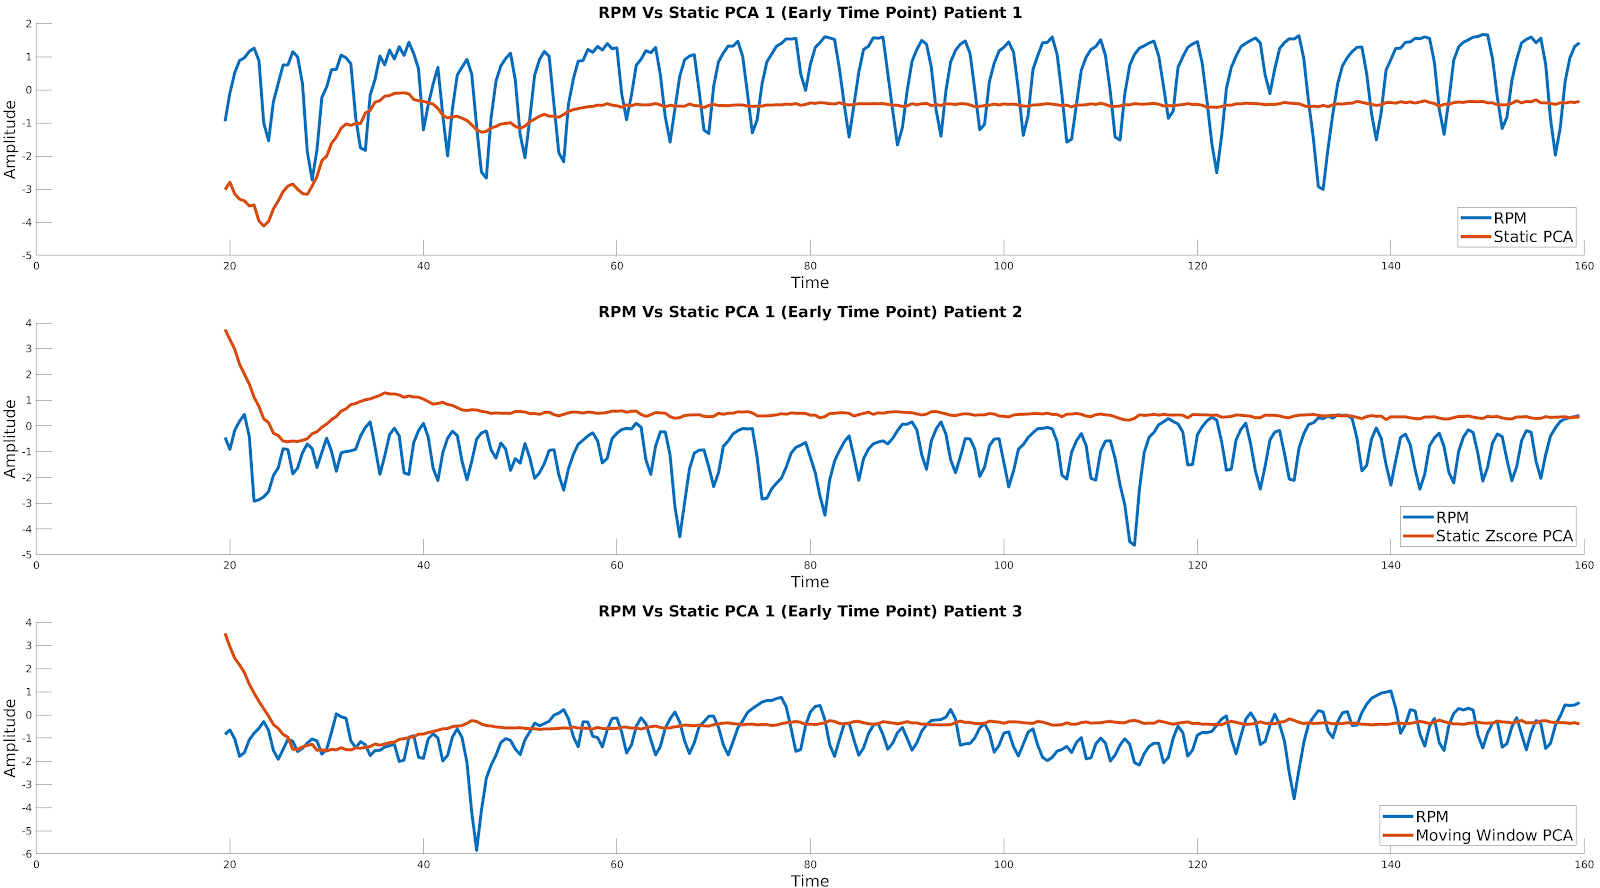
\includegraphics[width=1.0\linewidth]{figures/data_driven_surrogate_signal_extraction_results_1_vanilla_surrogate_signal.png}
                
                \captionsetup{singlelinecheck=false, justification=centering}
                \caption{A visual comparison between the \gls{RPM} \gls{SS} and the \gls{SS} from the static \gls{PCA} method using only the first \gls{PC} for three patients between \SI{20}{\second} and \SI{160}{\second}. The three patients shown here are the ones on which parameters for the method were optimised.}
                \label{fig:pca_data_driven_surrogate_signal_extraction_methods_for_dynamic_pet_results_vanilla_surrogate_signal}
            \end{figure}
            
            \begin{figure}
                \centering
                
                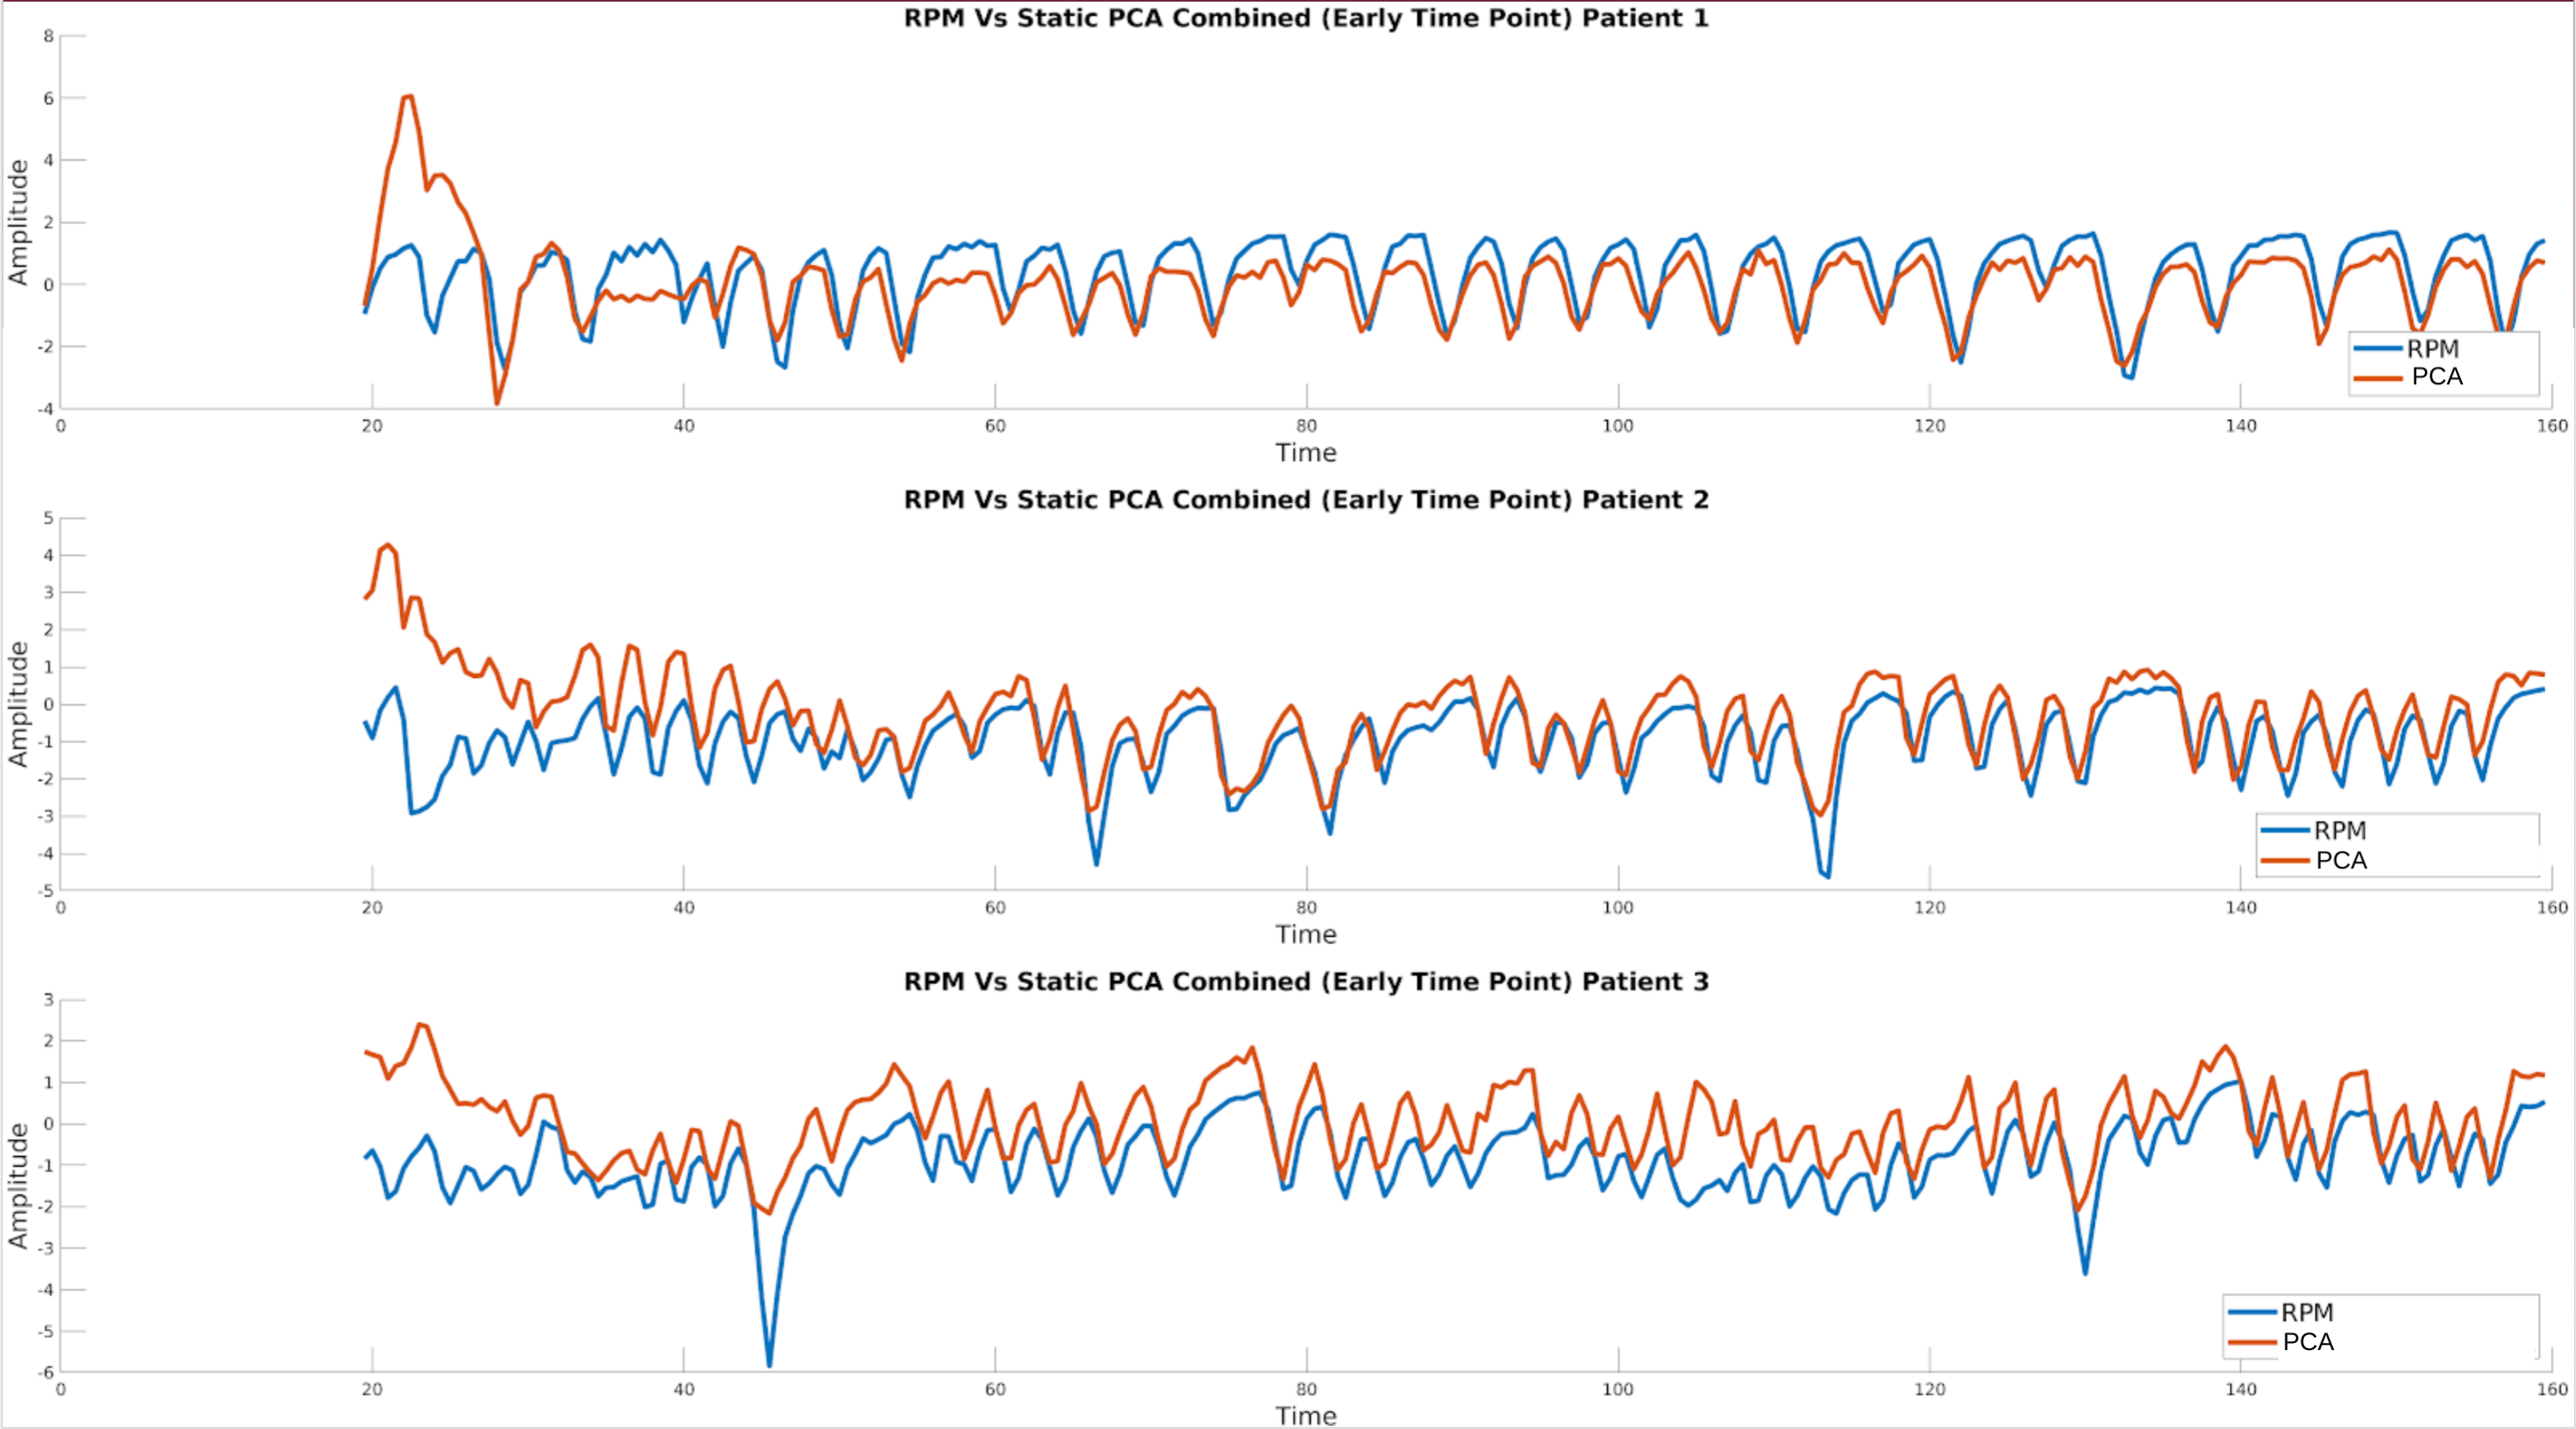
\includegraphics[width=1.0\linewidth]{figures/data_driven_surrogate_signal_extraction_results_1_combined_surrogate_signal.png}
                
                \captionsetup{singlelinecheck=false, justification=centering}
                \caption{A visual comparison between the \gls{RPM} \gls{SS} and the \gls{SS} from the static \gls{PCA} method by combining the first $20$ \glss{PC} for three patients between \SI{20}{\second} and \SI{160}{\second}. The three patients shown here are the ones on which parameters for the method were optimised. Here no pre or post-processing is used.}
                \label{fig:pca_data_driven_surrogate_signal_extraction_methods_for_dynamic_pet_results_combined_surrogate_signal}
            \end{figure}
            
            \begin{figure}
                \centering
                
                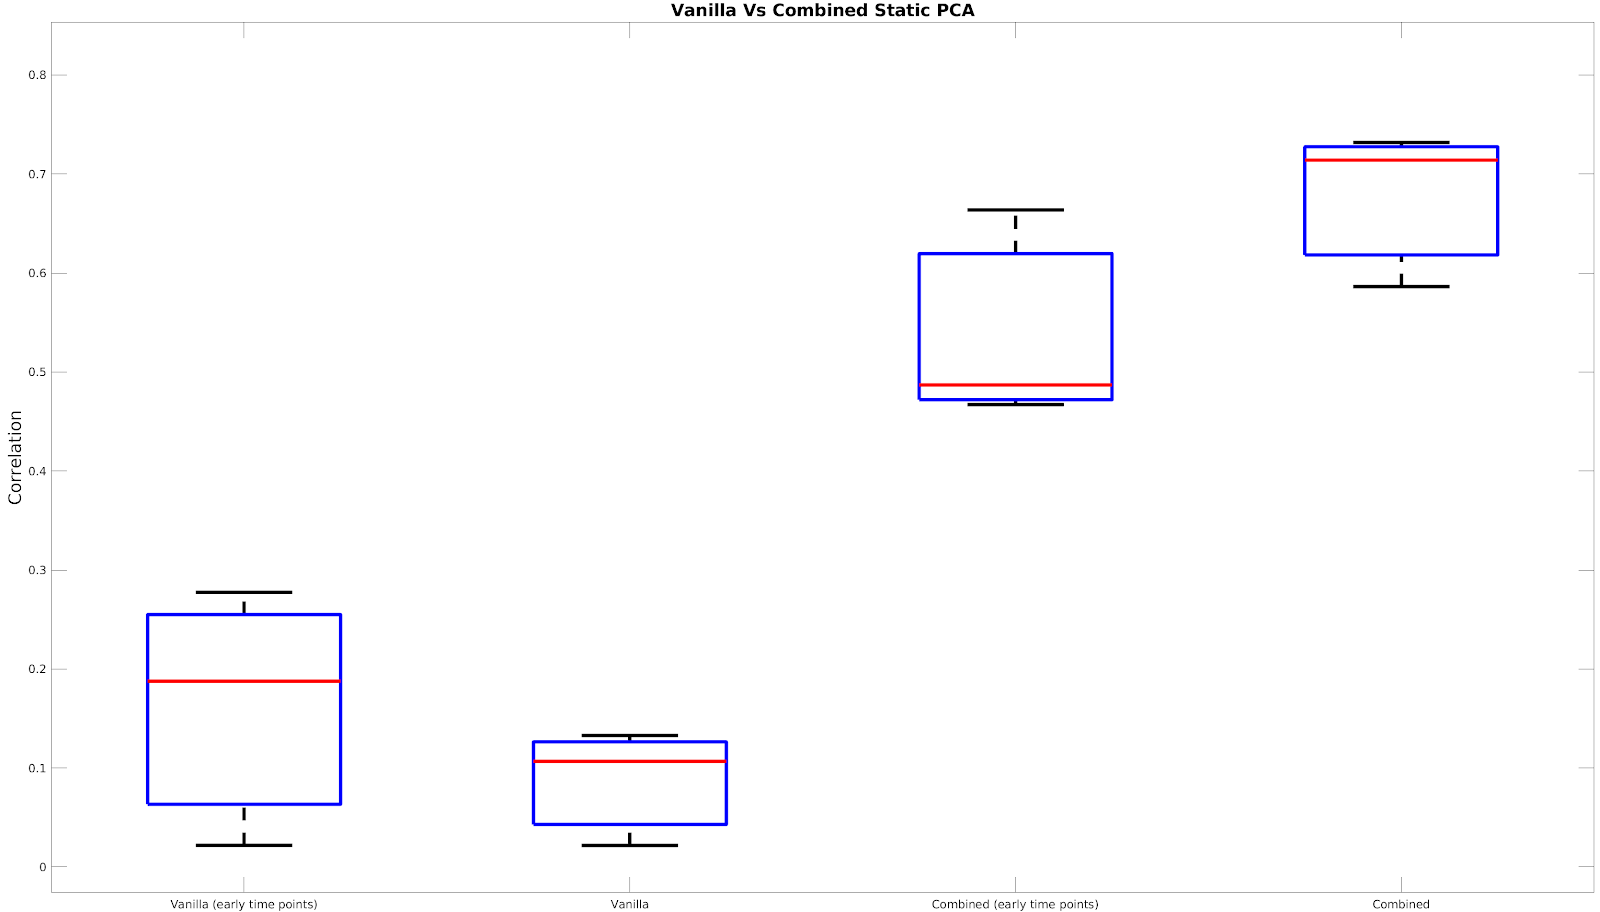
\includegraphics[width=1.0\linewidth]{figures/data_driven_surrogate_signal_extraction_results_1_box_plot.png}
                
                \captionsetup{singlelinecheck=false, justification=centering}
                \caption{A box plot of the \gls{CC} between static \gls{PCA} method both when using only the first \gls{PC} and by combining the first $20$ \glss{PC} for all patients between \SI{20}{\second} and \SI{160}{\second} and for the entire acquisition. The parameters used here were optimised for and frozen based on the results shown in other diagrams on three patients. Here no pre or post-processing is used.}
                \label{fig:pca_data_driven_surrogate_signal_extraction_methods_for_dynamic_pet_results_box_plot}
            \end{figure}
            
            \begin{figure}
                \centering
                
                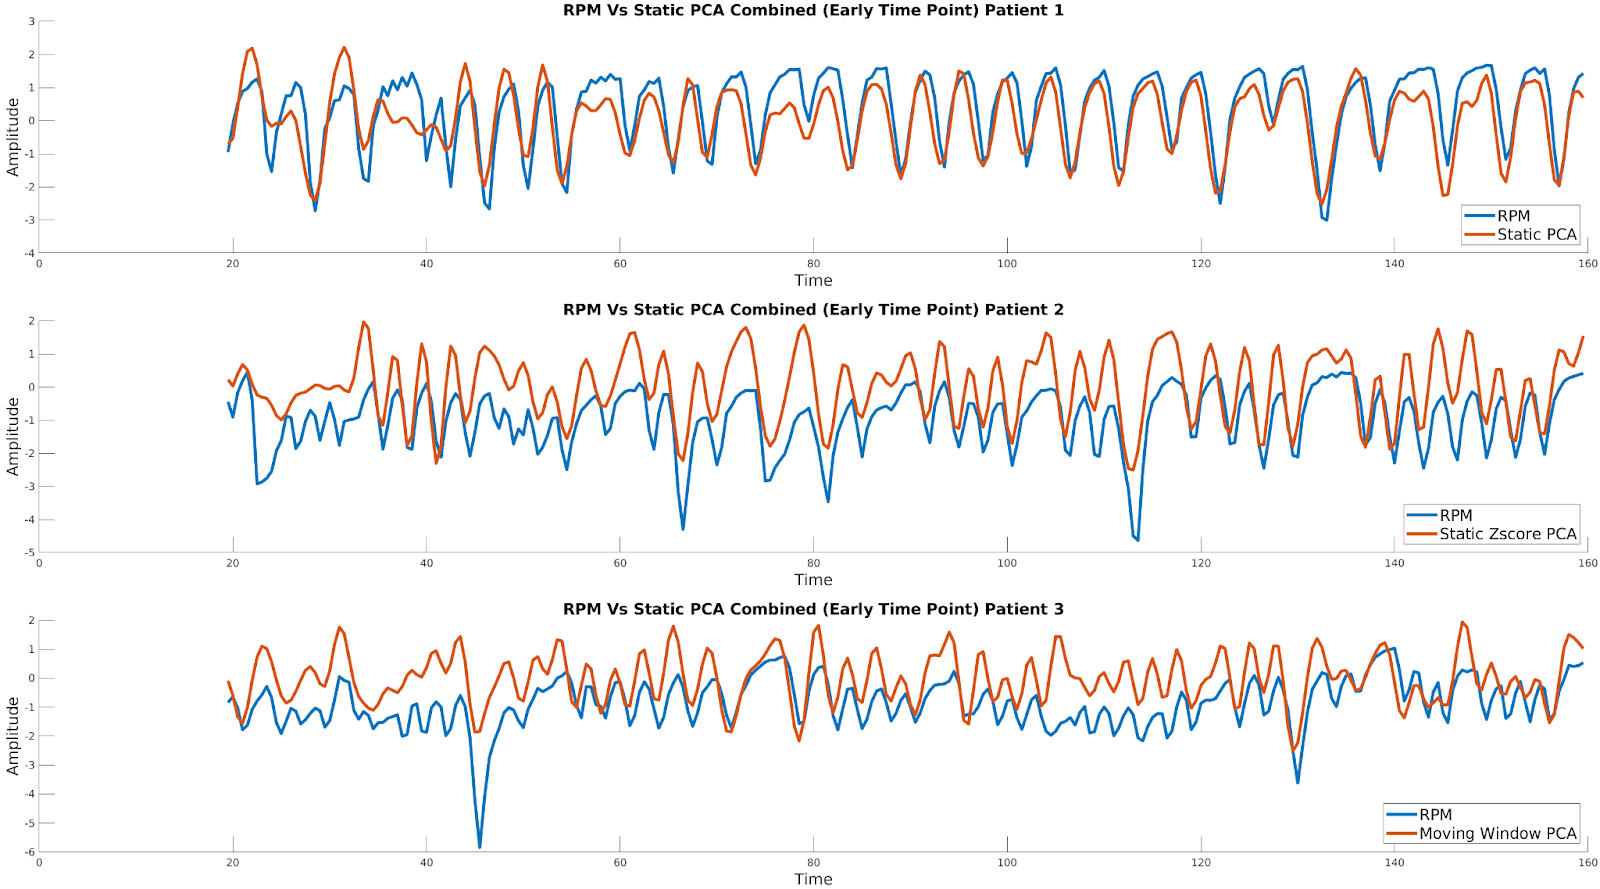
\includegraphics[width=1.0\linewidth]{figures/data_driven_surrogate_signal_extraction_results_1_combined_surrogate_signal_processed.png}
                
                \captionsetup{singlelinecheck=false, justification=centering}
                \caption{A visual comparison between the \gls{RPM} \gls{SS} and the \gls{SS} from the static \gls{PCA} method by combining the first $20$ \glss{PC} for three patients between \SI{20}{\second} and \SI{160}{\second}. The three patients shown here are the ones on which parameters for the method were optimised. Here pre and post-processing are used.}
                \label{fig:pca_data_driven_surrogate_signal_extraction_methods_for_dynamic_pet_results_combined_surrogate_signal_processed}
            \end{figure}
            
            \begin{figure}
                \centering
                
                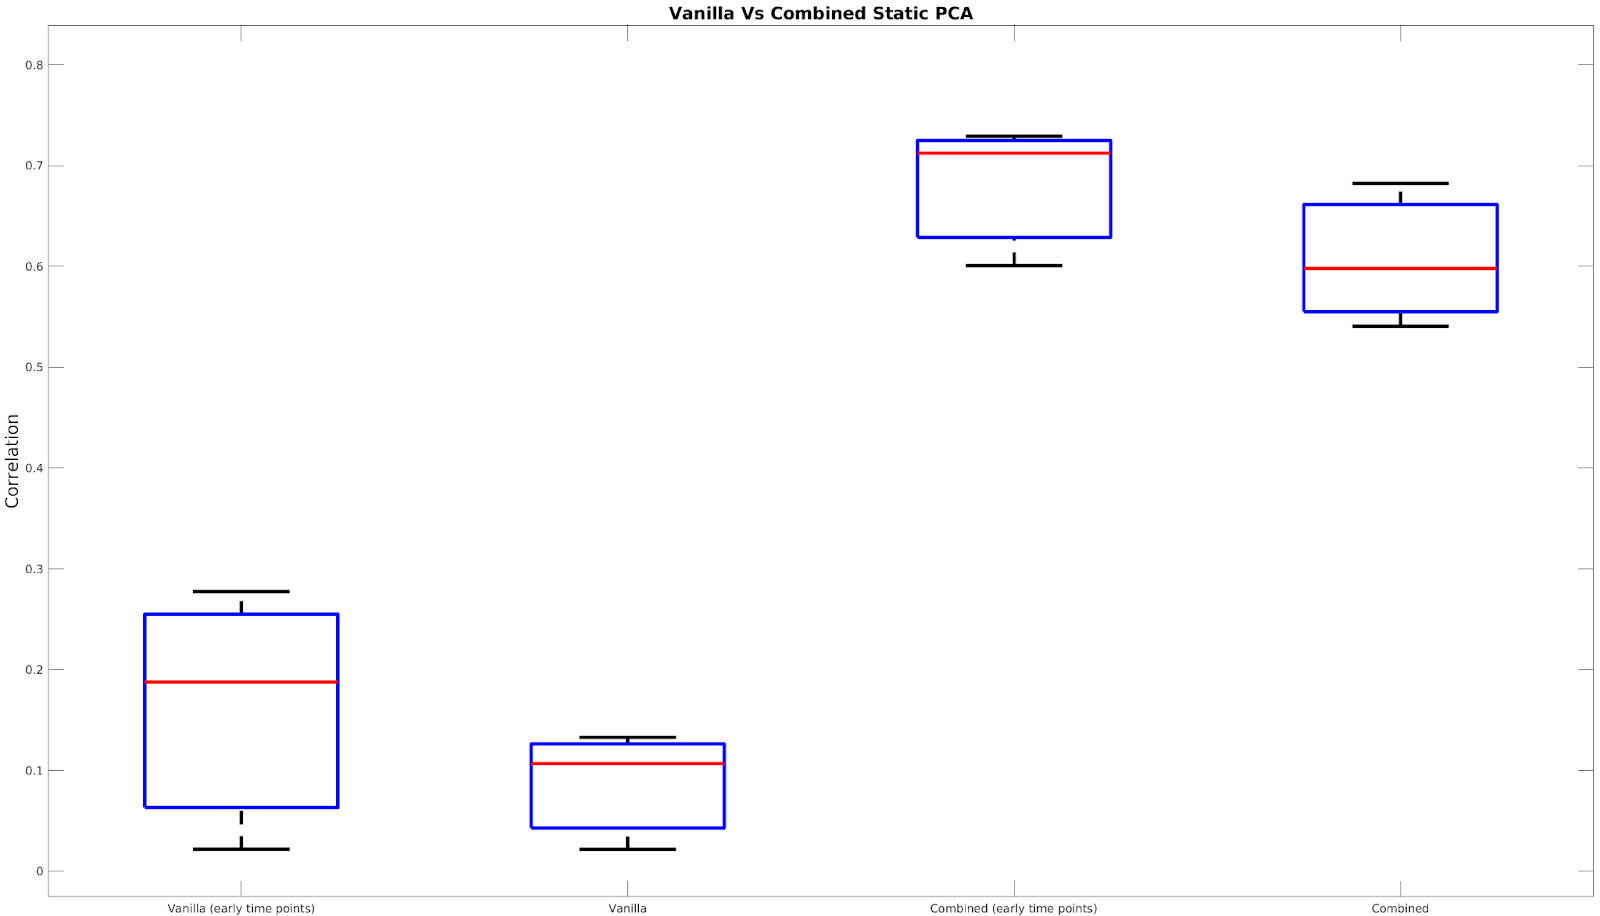
\includegraphics[width=1.0\linewidth]{figures/data_driven_surrogate_signal_extraction_results_1_box_plot_processed.png}
                
                \captionsetup{singlelinecheck=false, justification=centering}
                \caption{A box plot of the \gls{CC} between static \gls{PCA} method both when using only the first \gls{PC} and by combining the first $20$ \glss{PC} for all patients between \SI{20}{\second} and \SI{160}{\second} and for the entire acquisition. The parameters used here were optimised for and frozen based on the results shown in other diagrams on three patients. Here pre and post-processing are used.}
                \label{fig:pca_data_driven_surrogate_signal_extraction_methods_for_dynamic_pet_results_box_plot_processed}
            \end{figure}
            
            For results presented here parameters were selected on a subset of the data before being applied across the entire data set. A plot of the \gls{SS} for static \gls{PCA} using only one \gls{PC} for three patients at early time points can be seen in~\Fref{fig:pca_data_driven_surrogate_signal_extraction_methods_for_dynamic_pet_results_vanilla_surrogate_signal}. It can be observed in this example that only using the static \gls{PCA} method and one \gls{PC} does not give satisfactory results at early time points. A plot of the \gls{SS} for static \gls{PCA} using a combination of the first $20$ \glss{PC} for three patients at early time points can be seen in~\Fref{fig:pca_data_driven_surrogate_signal_extraction_methods_for_dynamic_pet_results_combined_surrogate_signal}, here no pre or post-processing is used. Here for all patients from very early in the acquisition it can be seen that the method gives comparable results to the \gls{RPM}. A plot of the \gls{SS} for static \gls{PCA} using a combination of the first $20$ \glss{PC} for three patients at early time points can be seen in~\Fref{fig:pca_data_driven_surrogate_signal_extraction_methods_for_dynamic_pet_results_combined_surrogate_signal_processed}, here pre and post-processing are used. The parameters for the processing were optimised solely to improve the \gls{CC} for early time points, as such it can be seen that some inter-window variation has been removed (from parallel compression).
            
            A box plot of the \gls{CC} of the \gls{SS} for static \gls{PCA} using only one \gls{PC} compared to the \gls{RPM} and the \gls{CC} of the \gls{SS} for static \gls{PCA} using a combination of the first $20$ \glss{PC} compared to the \gls{RPM} for all patients at both early time points and all time points and  can be seen in~\Fref{fig:pca_data_driven_surrogate_signal_extraction_methods_for_dynamic_pet_results_box_plot}, here no pre or post-processing is used. Here the improvement by incorporating multiple \glss{PC} is most apparent. A box plot of the \gls{CC} of the \gls{SS} for static \gls{PCA} using only one \gls{PC} compared to the \gls{RPM} and the \gls{CC} of the \gls{SS} for static \gls{PCA} using a combination of the first $20$ \glss{PC} compared to the \gls{RPM} for all patients at both early time points and all time points and  can be seen in~\Fref{fig:pca_data_driven_surrogate_signal_extraction_methods_for_dynamic_pet_results_box_plot_processed}, here pre and post-processing are used. The parameters for the processing were optimised solely to improve the \gls{CC} for early time points, as such it can be seen that the \gls{CC} drops from no processing to processing for the entire acquisition, it can be assumed this effect is similar to minimising variance at the expense of bias or vice versa.
            
        \subsection{Discussion and Conclusion} \label{sec:pca_data_driven_surrogate_signal_extraction_methods_for_dynamic_pet_discussion_and_conclusion}
            Results from a visual comparison of early time point signals from both an \gls{RPM} and static \gls{PCA} indicates that while using only one \gls{PC} leads to poor results the method of combining \glss{PC} presented here has good promise, this is further reinforced when the \gls{CC} is examined.
            
            In the future, research will focus on further development of the method, tuning the parameters of the additional methods to the point where they can be compared.
            
            However, the work presented here suffers from a few limitations. Firstly the data taken here all comes from the same study, using the same procedure, the same radiotracer and mostly acquired on the same scanner. In order to better validate the generalisability of the method it would be positive to test on data acquired on different scanners and using different radiotracers.
            
            An additional concern is that the method will fail for patients who exhibit abnormal breathing patters. For instance, extremely slow breathers will breath at a rate less than \SI{0.1}{\hertz}, which here would be considered to be tracer kinetics. Furthermore, the method struggles with patients who breath at less regular intervals, exemplified by those who occasionally hold their breath or otherwise stop breathing for periods and by those who breath in such a way as to induce multiple harmonics in their breathing, this could be seen as a signal atop a carrier. One method which could be developed to combat these issues would be to introduce machine learning, either to completely replace the method or to enhance it. A neural network could be added here to replace the three window method of selecting and combining \glss{PC}, a network could be trained to identify signals which are caused by respiration. There are already networks which are designed to discriminate between data, such as the aptly named discriminator network used as part of training a \gls{GAN}. 
    
%    \longsection{Feasibility Study of Neural Network Based Data Driven Surrogate Signal Extraction Methods for Dynamic PET}{sec:feasibility_study_of_neural_network_based_data_driven_surrogate_signal_extraction_methods_for_dynamic_pet}
        
        
%        \subsection{Introduction} \label{sec:feasibility_study_of_neural_network_based_data_driven_surrogate_signal_extraction_methods_for_dynamic_pet_introduction}
            
        
%        \subsection{Methods} \label{sec:feasibility_study_of_neural_network_based_data_driven_surrogate_signal_extraction_methods_for_dynamic_pet_methods}
            
            
%        \subsection{Results} \label{sec:feasibility_study_of_neural_network_based_data_driven_surrogate_signal_extraction_methods_for_dynamic_pet_results}
            
            
%        \subsection{Discussion and Conclusion} \label{sec:feasibility_study_of_neural_network_based_data_driven_surrogate_signal_extraction_methods_for_dynamic_pet_discussion_and_conclusion}
            
